\section{5 Dec 23 - Activity: Modeling the Ideal
Gas}\label{dec-23---activity-modeling-the-ideal-gas}

As we developed from
\href{https://github.com/dannycab/phy415msu/blob/main/MMIPbook/assets/pdfs/notes/Notes_4_Markov_Chain.pdf}{lecture},
we can sample the Boltzmann distribution by constructing a sample of it
through a Markov Chain and computing the value of the quantity of
interest and adding it up.

\[\sum_{chain} X_i \approx \langle X \rangle\]

\subsection{One Dimensional Gas}\label{one-dimensional-gas}

We will model an ideal gas, but let's start with a one-dimensional gas
made of a bunch of particles in infinite square wells. The energy
spectrum for a particle of mass \(m\) in an infinite square well of
length \(L\) is given by:

\[E(n) = \dfrac{\pi^2 \hbar^2}{2mL^2}n^2\]

We can simplify things by choosing \(\hbar\), \(\pi\), \(L\), and \(m\)
= 1. So that our energy is more simply written as:

\[E(n) = \dfrac{n^2}{2}\]

Our analysis relies on computing the change in energy in making one
quantum step \(n \pm 1\) and determining if we keep the step or not
based on the thermodynamic probability:

\[P = \exp(-\dfrac{\Delta E}{kT})\]

We take \(k=1\), so that:

\[P = e^{-\Delta E/T}\]

The change in energy as a result of moving the state up or down is given
by:

\[\Delta E_{down} = E(n-1) - E(n) = \dfrac{1}{2}\left((n-1)^2-n^2\right) = \dfrac{-2n+1}{2}\]

\[\Delta E_{up} = E(n+1) - E(n) = \dfrac{1}{2}\left((n+1)^2-n^2\right) = \dfrac{2n+1}{2}\]

\subsection{Implementation}\label{implementation}

Below is the code that develops a model of a one dimensional gas. It is
annotated. Review the code and make note of each piece of the algorithm.

\textbf{Complete the following}

\begin{enumerate}
\def\labelenumi{\arabic{enumi}.}
\tightlist
\item
  Run the simulation for a variety of temperatures. What do you notice?
\item
  Run the simulation for the same temperature and establish the average
  energy and uncertainty. Compare to the expected value.
\item
  Plot the histogram of final states. How does this look like a good
  sampling distribution?
\end{enumerate}

\begin{Shaded}
\begin{Highlighting}[]
\ImportTok{import}\NormalTok{ random }\ImportTok{as}\NormalTok{ random}
\ImportTok{import}\NormalTok{ numpy }\ImportTok{as}\NormalTok{ np}
\ImportTok{import}\NormalTok{ matplotlib.pyplot }\ImportTok{as}\NormalTok{ plt}
\OperatorTok{\%}\NormalTok{matplotlib inline}
\end{Highlighting}
\end{Shaded}

\begin{Shaded}
\begin{Highlighting}[]
\NormalTok{temperature }\OperatorTok{=} \DecValTok{10}
\NormalTok{numberOfAtoms }\OperatorTok{=} \DecValTok{1000}
\NormalTok{simulationSteps }\OperatorTok{=} \DecValTok{500000}

\NormalTok{quantumNumberArray }\OperatorTok{=}\NormalTok{ np.ones([numberOfAtoms,}\DecValTok{1}\NormalTok{], }\BuiltInTok{int}\NormalTok{)}

\NormalTok{energyAtEachStep }\OperatorTok{=}\NormalTok{ np.zeros([simulationSteps,}\DecValTok{1}\NormalTok{], }\BuiltInTok{float}\NormalTok{)}

\CommentTok{\#\# Each atom starts in n=1 and}
\CommentTok{\#\# Contributes 1/2 unit of energy (hbar, pi, m, L = 1)}
\NormalTok{E }\OperatorTok{=}\NormalTok{ numberOfAtoms}\OperatorTok{/}\DecValTok{2}

\CommentTok{\#\# Monte Carlo Loop}
\ControlFlowTok{for}\NormalTok{ step }\KeywordTok{in} \BuiltInTok{range}\NormalTok{(simulationSteps):}
    
    \CommentTok{\# Choose atom and the move}
\NormalTok{    ithAtom }\OperatorTok{=}\NormalTok{ random.randrange(numberOfAtoms)}
    
    \CommentTok{\# Randomly select the next energy state +1 or {-}1}
    \ControlFlowTok{if}\NormalTok{ random.random() }\OperatorTok{\textless{}} \FloatTok{0.5}\NormalTok{:    }
        
\NormalTok{        changeInState }\OperatorTok{=} \DecValTok{1}
\NormalTok{        changeInEnergy }\OperatorTok{=}\NormalTok{ (}\FloatTok{0.5}\NormalTok{)}\OperatorTok{*}\NormalTok{(}\DecValTok{2}\OperatorTok{*}\NormalTok{quantumNumberArray[ithAtom]}\OperatorTok{+}\DecValTok{1}\NormalTok{)}
    \ControlFlowTok{else}\NormalTok{:}
        
\NormalTok{        changeInState }\OperatorTok{=} \OperatorTok{{-}}\DecValTok{1}
\NormalTok{        changeInEnergy }\OperatorTok{=}\NormalTok{ (}\FloatTok{0.5}\NormalTok{)}\OperatorTok{*}\NormalTok{(}\OperatorTok{{-}}\DecValTok{2}\OperatorTok{*}\NormalTok{quantumNumberArray[ithAtom]}\OperatorTok{+}\DecValTok{1}\NormalTok{)}
        
    \CommentTok{\# Decide to accept with thermodynamic probability}
    \ControlFlowTok{if}\NormalTok{ quantumNumberArray[ithAtom] }\OperatorTok{\textgreater{}} \DecValTok{1} \KeywordTok{or}\NormalTok{ changeInState }\OperatorTok{==} \DecValTok{1}\NormalTok{:}
        
\NormalTok{        thermodynamicProbability }\OperatorTok{=}\NormalTok{ np.exp(}\OperatorTok{{-}}\NormalTok{changeInEnergy}\OperatorTok{/}\NormalTok{temperature)}
        
        \ControlFlowTok{if}\NormalTok{ random.random() }\OperatorTok{\textless{}}\NormalTok{ thermodynamicProbability:}
            
\NormalTok{            quantumNumberArray[ithAtom] }\OperatorTok{+=}\NormalTok{ changeInState}
\NormalTok{            E }\OperatorTok{+=}\NormalTok{ changeInEnergy}
    
\NormalTok{    energyAtEachStep[step] }\OperatorTok{=}\NormalTok{ E}
\end{Highlighting}
\end{Shaded}

\begin{Shaded}
\begin{Highlighting}[]
\NormalTok{plt.figure(figsize}\OperatorTok{=}\NormalTok{(}\DecValTok{8}\NormalTok{,}\DecValTok{6}\NormalTok{))}
\NormalTok{plt.plot(energyAtEachStep, label }\OperatorTok{=} \StringTok{\textquotesingle{}Simulated Energy\textquotesingle{}}\NormalTok{)}
\NormalTok{plt.hlines(numberOfAtoms}\OperatorTok{*}\NormalTok{temperature}\OperatorTok{/}\DecValTok{2}\OperatorTok{+}\NormalTok{numberOfAtoms}\OperatorTok{/}\DecValTok{2}\NormalTok{, }\DecValTok{0}\NormalTok{, simulationSteps, }\StringTok{\textquotesingle{}r\textquotesingle{}}\NormalTok{, label}\OperatorTok{=}\StringTok{\textquotesingle{}Equipartition Theorem + Ground State Energy\textquotesingle{}}\NormalTok{)}

\NormalTok{plt.ylabel(}\StringTok{\textquotesingle{}Energy\textquotesingle{}}\NormalTok{)}
\NormalTok{plt.xlabel(}\StringTok{\textquotesingle{}Steps\textquotesingle{}}\NormalTok{)}

\NormalTok{plt.grid()}
\NormalTok{plt.legend()}
\end{Highlighting}
\end{Shaded}

\begin{verbatim}
<matplotlib.legend.Legend at 0x11e621a80>
\end{verbatim}

\begin{figure}
\centering
\pandocbounded{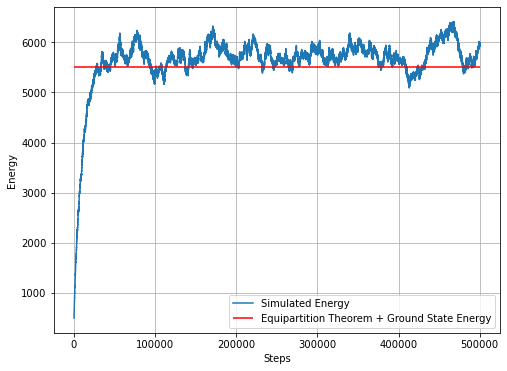
\includegraphics[keepaspectratio,alt={png}]{../images/activity-metropolis_activity-metropolis_tmp_4_1.png}}
\caption{png}
\end{figure}

\subsection{The Ideal Gas}\label{the-ideal-gas}

The code above can be used for an ideal gas. There are some changes you
have to make because an ideal gas in three dimensions has an energy
spectrum like this:

\[E(n_x,n_y,n_z) = \dfrac{\pi^2\hbar^2}{2mL^2}\left(n_x^2+n_y^2+n_z^2\right)\]

\textbf{Do this}

\begin{enumerate}
\def\labelenumi{\arabic{enumi}.}
\tightlist
\item
  Using the same approach (changing just one quantum number), find the
  value for \(\Delta E\) in general.
\item
  Sketch out how the code will need to change to accommodate three
  dimensions (Discuss with each other and Danny)
\item
  Implement those changes to calculate the energy of a 3D ideal gas.
\end{enumerate}

\begin{Shaded}
\begin{Highlighting}[]
\CommentTok{\#\# your code here}
\end{Highlighting}
\end{Shaded}

\begin{Shaded}
\begin{Highlighting}[]

\end{Highlighting}
\end{Shaded}
